\chapter{Implementación}

El proceso de hacer realidad este proyecto y poder tenerlo desplegado ha tenido diferentes pautas a seguir, empezando por la parte de ROS 2, ya que era la esencial en el funcionamiento de nuestra plataforma.

Tras esto se han ido añadiendo las diferentes secciones comentadas en el análisis, haciendo una breve descripción de porqué se ha escogido esa tecnología para cada tarea, además de los diferentes problemas encontrados al realizarlo.

\section{ROS 2}

Para la creación del proyecto es necesario tener instalado ROS 2 y todas sus dependencias, explicado en la documentación de su web \cite{ros2}. En este caso se ha utilizado la versión Foxy.

Además hay que añadir diferentes scripts a nuestra shell para poder ejecutar los programas, o tener disponible el autocompletado de los comandos. Tras la instalación y configuración, se puede ejecutar algún programa de ejemplo para probar si se ha completado todo de manera correcta. 

ROS 2 trae diferentes herramientas, donde se van a destacar las más utilizadas en el proyecto:

\begin{itemize}
    \item \textbf{ros2 command}. Utilizado para diferentes tareas como ejecutar programas de ros2, creación de paquetes, consultar información de los nodos en ejecución, consulta de tópicos y más para cosas relacionadas con la parte de depuración.
    \item \textbf{colcon}. Utilizado para compilar el proyecto de ros, pudiendo seleccionar los diferentes paquetes por si está dividido en diferentes secciones.
    \item \textbf{rqt\_graph}. Herramienta gráfica que genera un esquema de la red con los diferentes nodos y tópicos, con sus respectivas conexiones, pudiendo mostrar u ocultar según unos parámetros a seleccionar.
\end{itemize}

Por lo tanto, para empezar se va a crear el entorno de trabajo, creando una carpeta para ello y tras esto, crear un directorio \textit{src} en su interior. Ahí tras ejecutar \verb|colcon build| que genera las diferentes carpetas necesarias se podrán crear los diferentes paquetes.

\subsection{Creación de las diferentes interfaces utilizadas en los tópicos}

Para poder utilizar los tópicos definidos en el análisis, es necesario crear un paquete donde se van a implementar esas interfaces. Para ello, situado en el directorio \verb|workdir/src| se ejecutaría el comando para crear un paquete, \verb|ros2 pkg create my_tfg_interfaces|.

Tras esto, será generada la carpeta \verb|my_tfg_interfaces|, donde se será necesario crear los diferentes directorios y ficheros, para tener una estructura similar a la siguiente:
\begin{lstlisting}[language=Bash, caption=Estructura del directorio de trabajo]
src/my_tfg_interfaces/
    msg/
        FloatDataNode.msg
        StatusNode.msg
        Position.msg
    srv/
        UploadFile.srv
    CMakeLists.txt
    package.xml
\end{lstlisting}

Tras esto, el código de los archivos creados \textit{.msg} y \textit{.srv} es muy simple, por lo que vamos a visualizar \verb|FloatDataNode.msg|:

\lstinputlisting[language=C, caption=Código FloatDataNode.msg]{code/FloatDataNode.msg}

Como se puede observar, solo hay que declarar las variables que se quieran utilizar en el envío. Esto es debido al uso de IDL, que solo hace necesario la definición de estas, ya que ROS genera los diferentes ficheros necesarios. Por aclarar,  \verb|Position| en este caso es otro archivo, como si fuese un objeto con las otras variables.

En el caso de los servicios, el formato cambia un poco ya que hay un \textit{request} y un \textit{reply}, por lo tanto se escribe dividido como en el ejemplo a continuación:

\lstinputlisting[language=C, caption=Código UploadFile.srv]{code/UploadFile.srv}

Este código corresponde a \verb|UploadFile.srv|, utilizado en la comunicación del nodo controlador y el nodo gestor de la base de datos.

Tras esto sería necesario modificar los archivos \textbf{CMakeList.txt} y \textbf{package.xml}, añadiendo las dependencias correspondientes y los archivos creados.

Por último, tras cada nuevo elemento o modificación de cada paquete, es necesario volver a compilar cada paquete. 

\subsection{Desarrollo de los nodos}

Al igual que se ha creado un paquete en el punto anterior, en este caso se aplicaría el mismo procedimiento, pero el comando no sería exactamente el mismo, ya que sería necesario indicar el tipo de lenguaje a utilizar.

Como lenguaje se va a utilizar Python, aunque sería posible utilizar otros lenguajes, como C++. Por lo tanto para generar el paquete ejecutamos:

\begin{lstlisting}[language=Bash, caption=Comando para la creación de un paquete de Python con ROS 2]
ros2 pkg create my_tfg_pkg --build-type ament_python \
--dependencies rclpy
\end{lstlisting}

Esto es para la creación del paquete especificando el tipo de lenguaje y las dependencias, en este caso \textit{rclpy} que contiene todo lo necesario para poder desarrollar los nodos.

Tras todo esto, el directorio tendría la siguiente estructura:

\begin{lstlisting}[language=Bash, caption=Estructura del directorio de desarrollo con Python]
src/my_tfg_pkg/
    my_tfg_pkg/
        __init__.py
    test/
    resource/
    setup.cfg
    setup.py
    package.xml
\end{lstlisting}

Para poder construir los diferentes nodos, tenemos que añadir los respectivos ficheros en la carpeta \verb|src/my_tfg_pkg/my_tfg_pkg|.

Antes de empezar con la implementación, según la comunidad, la estructura estándar de los nodos tiene que ser la siguiente:

\newpage

\lstinputlisting[language=Python, caption=Plantilla genérica para la creación de nodos]{code/template-node.py}


Se puede observar en el código un método \textit{main} donde se crea un objeto de nuestra clase, y con el método \textit{spin}, se mantiene en ejecución ese nodo. Con esta base ya se pueden empezar a crear los nodos necesarios.

Por tanto, se va a repasar los diferentes nodos de manera genérica:

\begin{itemize}
    \item \textbf{Sensores.} Productores de información.
    \item \textbf{Actuadores.} Consumidores de esos datos, y productores de otros.
    \item \textbf{Controladores.} Encargados de recopilar todos los datos.
\end{itemize}

En las figuras mostradas durante el análisis, podemos observar el diseño definido de estos archivos concretamente en la \ref{fig:diagrama-clases}.

\subsubsection{Sensores}

Van a realizar una lectura del sensor cada cierto tiempo, llamando al método \verb|read_sensor()|. Esta función será la principal diferencia entre este tipo de nodo, ya que para su implementación será necesario una librería u otra. Tras esta lectura, estos datos serán publicados en la red. Para ello es necesario tener:

\begin{itemize}
    \item Un \textbf{publisher}, que defina el tópico donde se va a publicar
    \item Un \textbf{timer}, que establezca el tiempo cada vez que se va a realizar esa publicación. Este tendrá como parámetro la función de \verb|publish_value()|, que será llamada en el periodo definido.
\end{itemize}

Su declaración viene explicada en la documentación \cite{ros2}, pero por abreviar la búsqueda, esta se realiza de la siguiente forma:

\begin{lstlisting}[language=Python, caption=Publisher del sensor de temperatura]
self.temperature_publisher_ = 
    self.create_publisher(FloatDataNode, "temperature", 10)
self.sensor_timer_ = 
    self.create_timer(20.0, self.publish_temperature_data)
\end{lstlisting}

Se va a definir el \verb|publisher|, ya que los argumentos pueden ser confusos:

\begin{itemize}
    \item \textbf{FloatDataNode}, hace referencia al tipo de dato publicado en el tópico
    \item \textbf{"temperature"}, es el nombre del tópico donde se van a publicar los datos
    \item \textbf{10}, hace referencia al número de mensajes a conservar en el historial. También se puede declarar un elemento QoSProfile donde declaremos las diferentes QoS \cite{qos-ros} a aplicar.
\end{itemize}

El \verb|timer| recibe como parámetros el tiempo y la función que va a llamar, donde el \verb|publisher| publica el mensaje.

Según el los diferentes tipos de sensores que tenga conectados este nodo, le será necesario ese mismo número de \verb|publishers| con sus respectivas funciones.

\subsubsection{Actuadores}

A diferencia de los sensores, estos van a tener un \verb|publisher| para el estado de este nodo, el \verb|timer| para la publicación de esta información y un \verb|subscriber|.

Este \verb|subscriber| es el nuevo añadido a diferencia del anterior nodo. Para ver su estructura vamos a visualizar la siguiente declaración:

\begin{lstlisting}[language=Python, caption=Subscriber del actuador]
self.temperature_subscriber_ = self.create_subscription(
  FloatDataNode, "temperature", self.callback_sensor_data, 10)
\end{lstlisting}

Los parámetros hacen referencia al tópico del que se quieren leer los datos. El método \verb|callback_sensor_data| maneja los datos recibidos, comparando la temperatura en este caso con un posible valor de acción. Como se comenta en la parte de análisis, un ejemplo es cuando la temperatura baje de 12ºC, la calefacción se encienda y tras esto, se publique el nuevo estado.

\subsubsection{Controladores}

El nodo \textbf{controlador} posee más funcionalidades que los anteriores, ya que está orientado a utilizarse en un dispositivo central con más potencia.

Posee un \verb|subscriber| por cada tipo de tópico en la red, y tras la recepción de cada dato es guardado en un diccionario de Python. Este diccionario tras un tiempo definido con un timer almacena los datos en un json, para posteriormente contactar con el nodo gestor de la base de datos. Esto lo hace en los dos métodos siguientes

\begin{lstlisting}[language=Python, caption=Creación de cliente de ROS2 en Python]
def call_upload_file(self, json_name):
    client = self.create_client(UploadFile, "upload_db")
    while not client.wait_for_service(1.0):
        self.get_logger().warn("Waiting for DB Service...")

    request = UploadFile.Request()
    request.device_id = self.status_controller_.device_id
    request.filename = json_name

    future = client.call_async(request)
    future.add_done_callback(
        partial(self.callback_upload_file,
                device_id=self.status_controller_.device_id,
                filename=json_name))

def callback_upload_file(self, future, device_id, filename):
    try:
        response = future.result()
        if response.success:
            self.get_logger().info("Upload to Database done.")
    except Exception as e:
        self.get_logger().error("Service failed %r" % (e,))
\end{lstlisting}

Aquí se está gestionando una comunicación cliente-servidor, debido a que pub-sub no es la más indicada en este caso, ya que es necesario la obtención de respuesta por parte del gestor de la base de datos.

Se pueden visualizar métodos asíncronos ya que no se puede detener la ejecución del controlador de almacenar los demás datos que llegan en ese tiempo.

Por estructurar el código mostrado, primeramente se crea el cliente según el tópico a utilizar y se espera una conexión por parte del servidor. Tras esto se crea el objeto request que va a ser enviado. Por último se realiza la espera asíncrona de la response, y según su valor, se muestra en el gestor de logs que ha sido subido o se lanza una excepción.

\subsubsection{Ejecución y herramientas utilizadas}

Terminando esta sección se van a mostrar en las siguientes capturas la ejecución de los nodos, diferentes herramientas en la shell con el comando ros2, y por último el estado de la red mostrado con rqt\_graph.

\newpage

 \begin{center}
    \centering
    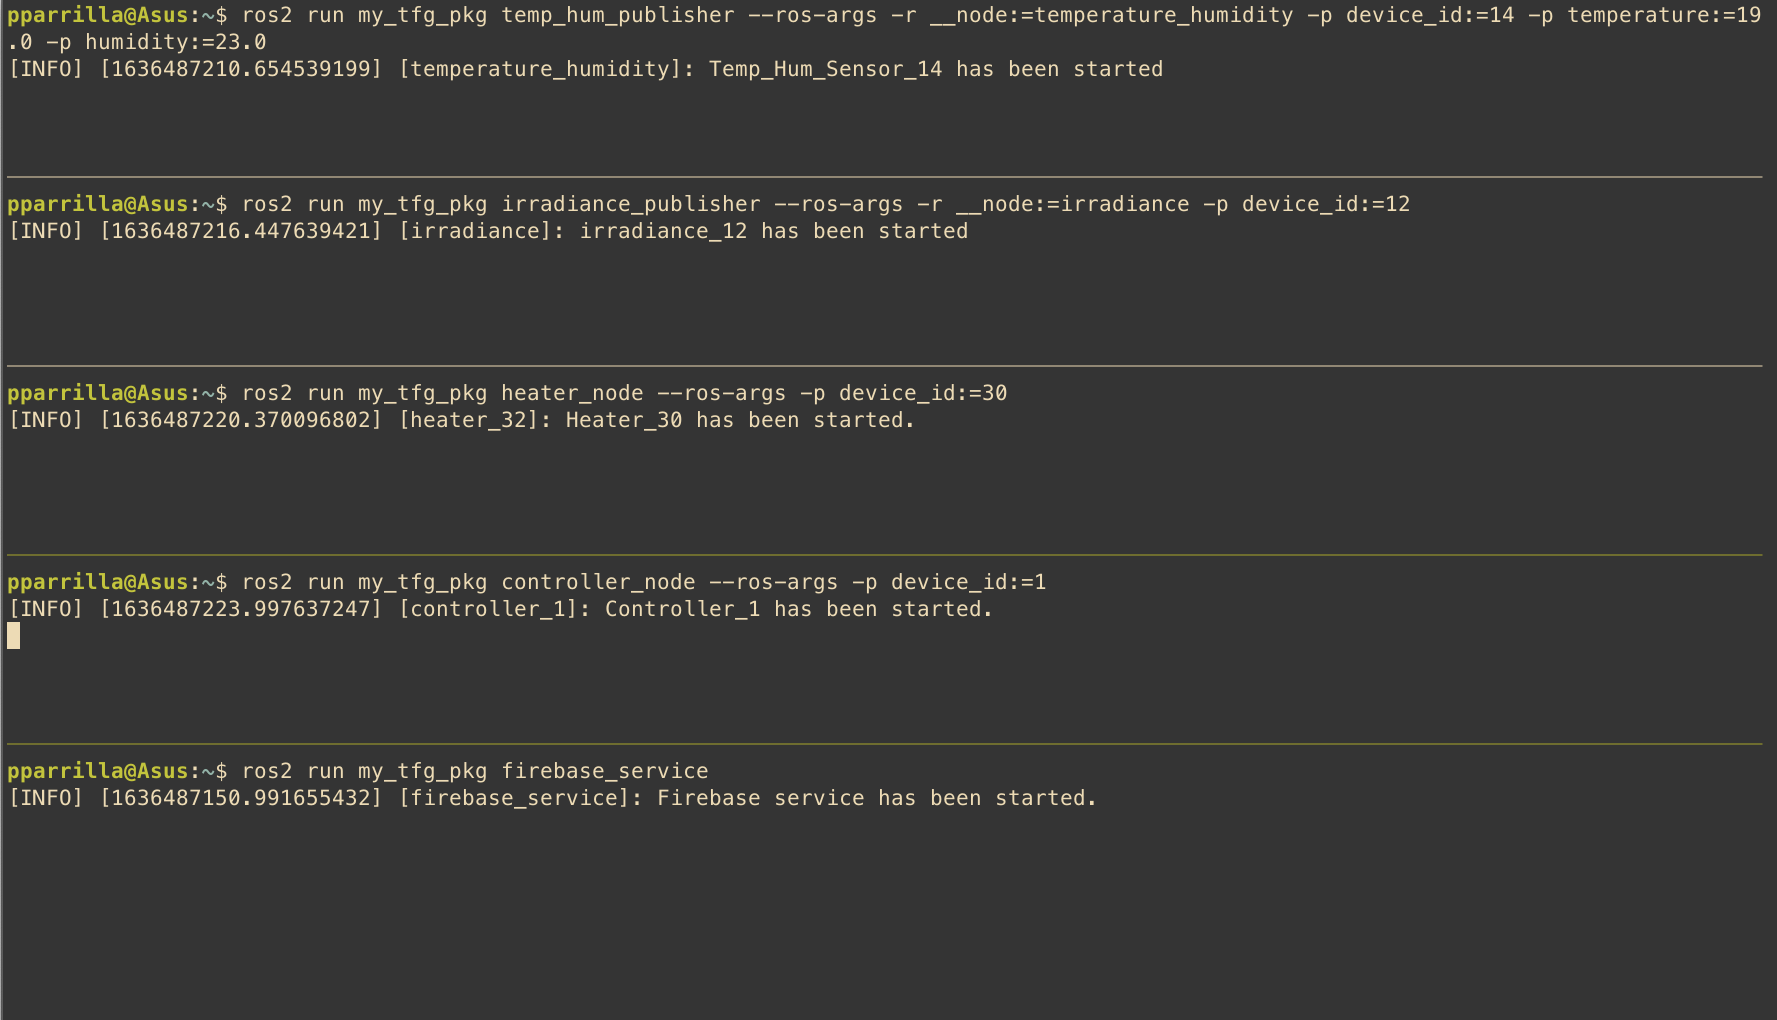
\includegraphics[width=\textwidth]{img/06-Ejecucion-nodos.png}
    \captionof{figure}{Ejecución de los diferentes nodos con parámetros}
    \label{fig:ejecucion-nodos}
\end{center}

Estos parámetros hacen referencia al id del dispositivo o al valor de temperatura que va a estar emitiendo ese nodo, ya que actualmente son virtuales y no leen de ningún sensor físico.

 \begin{center}
    \centering
    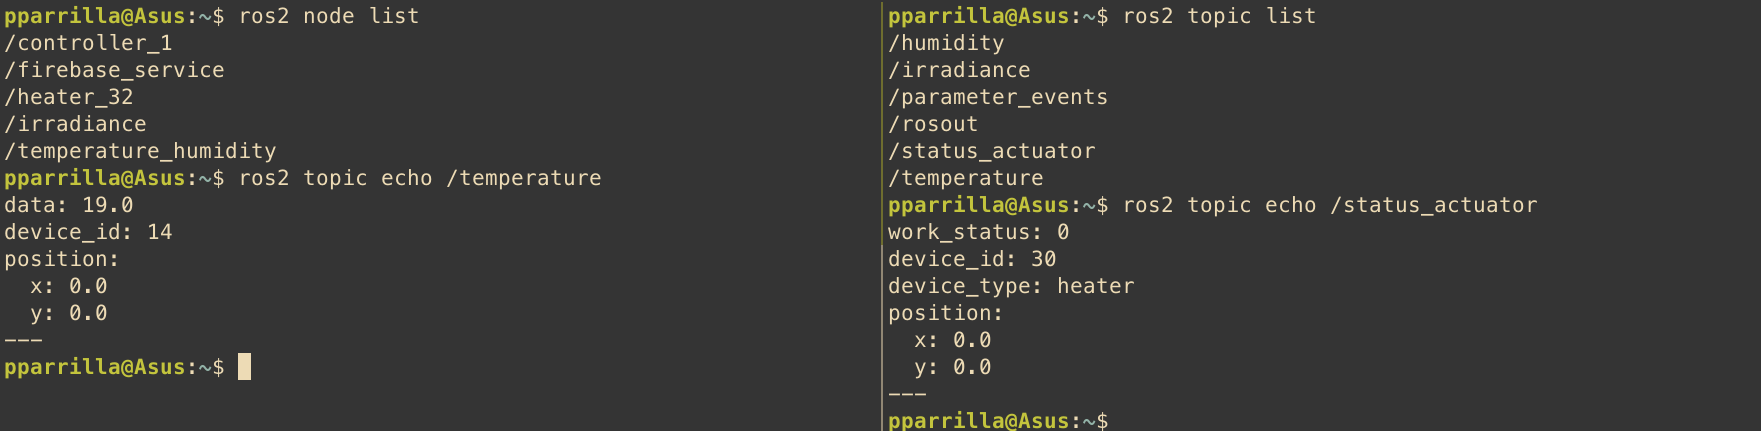
\includegraphics[width=\textwidth]{img/06-Tools.png}
    \captionof{figure}{Herramientas con el comando ros2}
    \label{fig:tools-ros2}
\end{center}

Se pueden observar distintos comandos de ros2 en la anterior figura:

\begin{itemize}
    \item \textbf{ros2 node list} muestra la lista de nodos actualmente ejecutandose en la red
    \item \textbf{ros2 topic list} muestra la lista de tópicos en la red
    \item \textbf{ros2 topic echo /temperature} muestra por pantalla los datos publicados referentes a ese tópico de temperatura
\end{itemize}

Hay más comandos similares, como \verb|ros2 interfaces show interface.msg| que mostraría las variables que implementa esa interfaz, muy útil cuando se utilizan interfaces no propias. Pero los más utilizados son los mostrados en la figura \ref{fig:tools-ros2}.

 \begin{center}
    \centering
    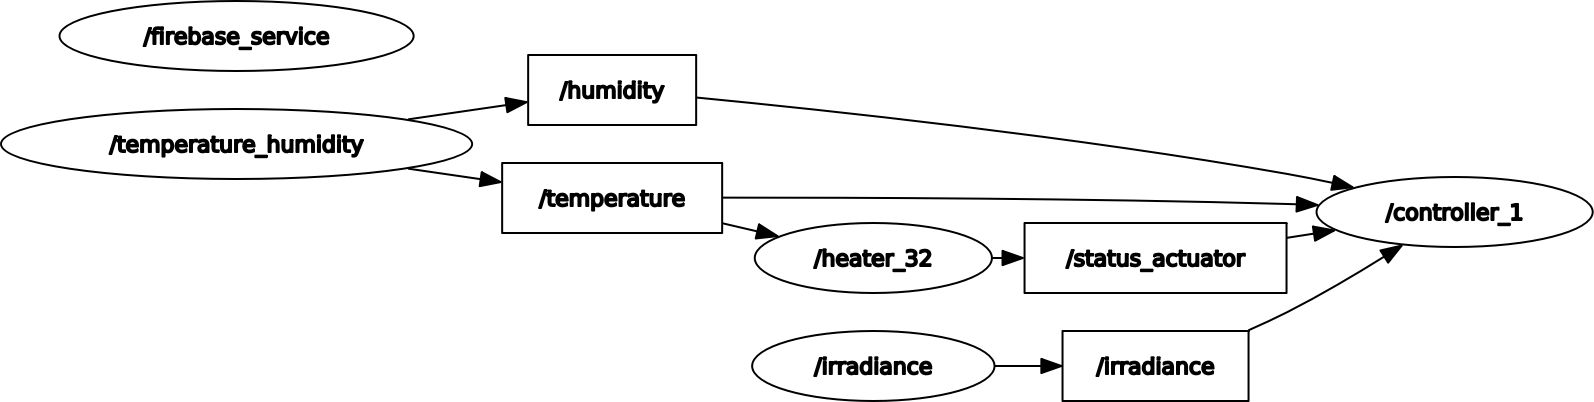
\includegraphics[width=\textwidth, height=4.5cm]{img/06-Rosgraph.png}
    \captionof{figure}{Gráfico generado con rqt-graph de la red}
    \label{fig:rqt-graphs}
\end{center}

Por aclarar al igual que en la figura \ref{fig:diagrama-comunicacion-nodos} los nodos están representados con el óvalo, y los rectángulos son los tópicos.

Esta herramienta, como se ha comentado, genera un gráfico de los distintos nodos y tópicos ejecutandose en la red, mostrando la comunicación existente. Los tópicos utilizados en conexiones cliente-servidor no los añade a la red, por eso \verb|controller_1| y \verb|firebase_service| no aparecen conectados.


\subsection{Micro ROS en microcontroladores}

Además de la utilización de ROS 2 en este proyecto, se han querido utilizar microcontroladores ya que son utilizados en casi cualquier producto robótico, estas tienen una baja latencia en cuestión a trabajo a tiempo real y consumen menos energía, además de su precio que suele ser más económico.

Para ello, es necesario la utilización de micro-ROS \cite{micro-ros}, que es la adaptación de la tecnología a estos microcontroladores. Además ha sido necesario utilizar FreeRTOS \cite{free-rtos}. Esto es un sistema operativo a tiempo real donde encima se va a ejecutar micro-ROS.

Una vez preparado el entorno como viene explicado en la documentación de micro-ROS, es necesario crear los siguientes ficheros:

\begin{itemize}
    \item \textbf{app.c}, que contiene la aplicación que se va a ejecutar
    \item \textbf{app-colcon.meta}, que contiene la información especifica necesaria para la compilación con \textit{colcon}.
\end{itemize}

Como se puede observar, ahora hay que utilizar C como lenguaje, donde no existen las clases, por tanto la estructura del fichero va a variar, pero no mucho ya que se realizará la mayoría de cosas en el propio main, llamando a diferentes métodos.

El objetivo va a ser utilizando una placa ESP32 leer de un sensor DHT-11 la temperatura y humedad, por lo tanto es necesario también incluir en el proyecto la librería especifica para realizar la lectura de datos.

La creación de un publisher y un timer en este caso ha sido la siguiente:

\begin{lstlisting}[language=C, caption=Publisher Timer y Executor en C para microcontrolador]
// create publisher for temperature
RCCHECK(rclc_publisher_init_default(
        &temperature_publisher,
        &node,
        ROSIDL_GET_MSG_TYPE_SUPPORT(custom_node_message, msg, 
                                        FloatDataNode),
        "temperature"));
        
// create timer
rcl_timer_t timer;
const unsigned int timer_timeout = 30000;
RCCHECK(rclc_timer_init_default(
        &timer,
        &support,
        RCL_MS_TO_NS(timer_timeout),
        timer_callback));

// create executor
rclc_executor_t executor;
RCCHECK(rclc_executor_init(&executor, 
                        &support.context, 1, &allocator));
RCCHECK(rclc_executor_add_timer(&executor, &timer));
\end{lstlisting}

Tras esto, cada 30 segundos se ejecuta la función \verb|timer_callback| que se encarga de leer los datos del sensor y publicarlos.

Ya con la aplicación operativa y todas las dependencias añadidas, sería momento de construir el proyecto y flashearlo en el microcontrolador.

El montaje del sensor y la placa tendría la siguiente estructura:

\newpage

 \begin{center}
    \centering
    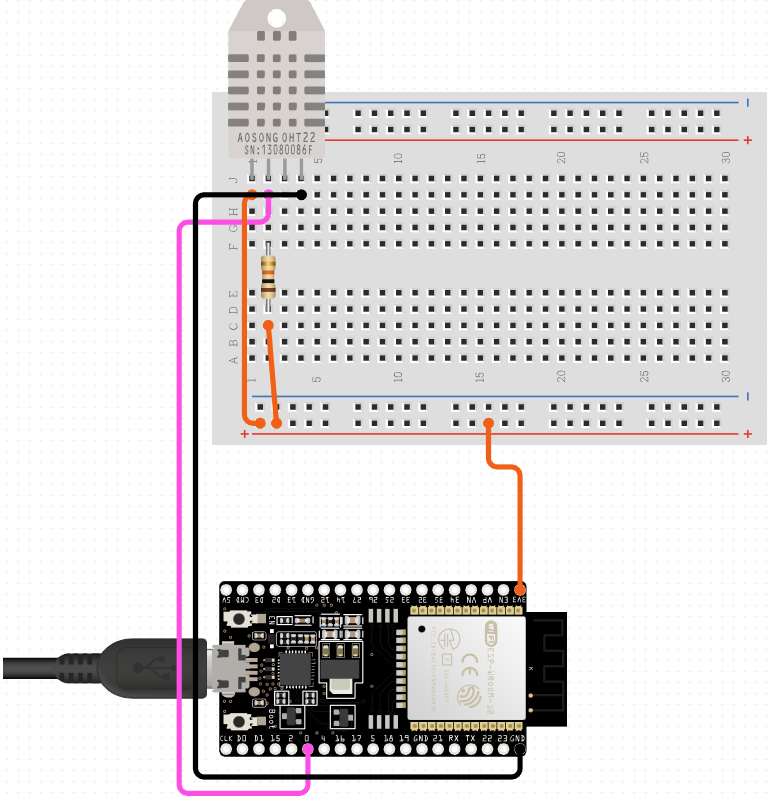
\includegraphics[width=0.6\textwidth]{img/06-DiagramaESP32.png}
    \captionof{figure}{Montaje ESP32 con DHT11}
    \label{fig:esp32-dht11}
\end{center}

Hay que tener en cuenta, que micro-ROS necesita la existencia de un agente para que el microcontrolador pueda contactar con el resto del proyecto de ROS 2. Este puede ser ejecutado en un contenedor de Docker \cite{docker} con el siguiente comando:

\begin{lstlisting}[language=Bash, caption=Ejecución Agente de micro-ROS en un contenedor Docker]
docker run -it --rm --net=host microros/micro-ros-agent:foxy \ 
    udp4 --port 8888 -v6
\end{lstlisting}

Este contenedor debería estar ejecutando en uno de los controladores distribuidos por el escenario, o en otro dispositivo dedicado para ello.

\subsection{Conexión a la base de datos}

Como se ha comentado, cada controlador almacena la información en un fichero tipo .json, y tras esto contacta con el gestor de la base de datos mediante cliente-servidor. Para ello tiene que enviar su id y el nombre el fichero.

Por lo tanto, el nodo de conexión a la base de datos debe tener las librerias para poder conectarse a esta.

En este caso se han implementado 2 nodos diferentes:

\begin{itemize}
    \item \textbf{Nodo Firebase.} Este realiza una conexión con Firebase \cite{firebase}, donde el archivo será estructurado en colecciones y documentos según define esta tecnología. El motivo a utilizar esta base de datos es el alojamiento en la nube, ya que facilita el acceso a los datos mediante las distintas plataformas. La librería para poder realizar la conexión es \textit{firebase\_admin}.
    \item \textbf{Nodo SQLite3.} Este crea una conexión con SQLite3 \cite{sqlite3} donde se almacenarán los datos de manera local del dispositivo en formato de tablas. Este puede estar ejecutado en cada dispositivo donde se ejecuta el nodo controlador, pudiendo tener la información replicada. La librería para poder realizar la conexión es \textit{sqlite3}.
\end{itemize}

En cada nodo es necesario presentar una estructura de creación del servidor, método para gestionar la llamada y otro método para subir la información a las respectivas bases de datos. 
% Todo este código puede ser visualizado haciendo click \href{https://github.com/pparrilla/ROS2_TFG/blob/main/src/my_tfg_pkg/my_tfg_pkg/firebase_service.py}{aquí}.

La explicación para el uso de dos bases de datos distintas...


\subsection{Simulación de un entorno con diferentes nodos}

Tras haber implementado los diferentes nodos, en caso de realizar una simulación del escenario descrito, no es viable la opción de ejecutar cada nodo de manera individual en una terminal como se muestra en la figura \ref{fig:ejecucion-nodos}, ya que en este caso se quieren lanzar unos 15-20 nodos aproximadamente.

Para estas ocasiones, ROS 2 dota de un tipo de archivo llamado \textit{Launch File}. En este se pueden incluir los diferentes nodos que se quieren ejecutar, indicando los parámetros como el nombre, el valor a producir, la posición y los demás que se hayan asignado durante el desarrollo de estos.

Por lo tanto da la posibilidad de generar un escenario y ejecutarlo desde un fichero, con el comando \textit{ros2 launch}.

Para su uso sería necesario la creación de otro paquete al igual que en los anteriores casos, y tras esos en un archivo tipo \textit{name.launch.py} escribir el código necesario, importanto la libreria \textit{launch}.

Tras el desarrollo y la ejecución de este fichero, con \textit{rqt\_graph} podemos observar la red de la siguiente forma:

\newpage

 \begin{center}
    \centering
    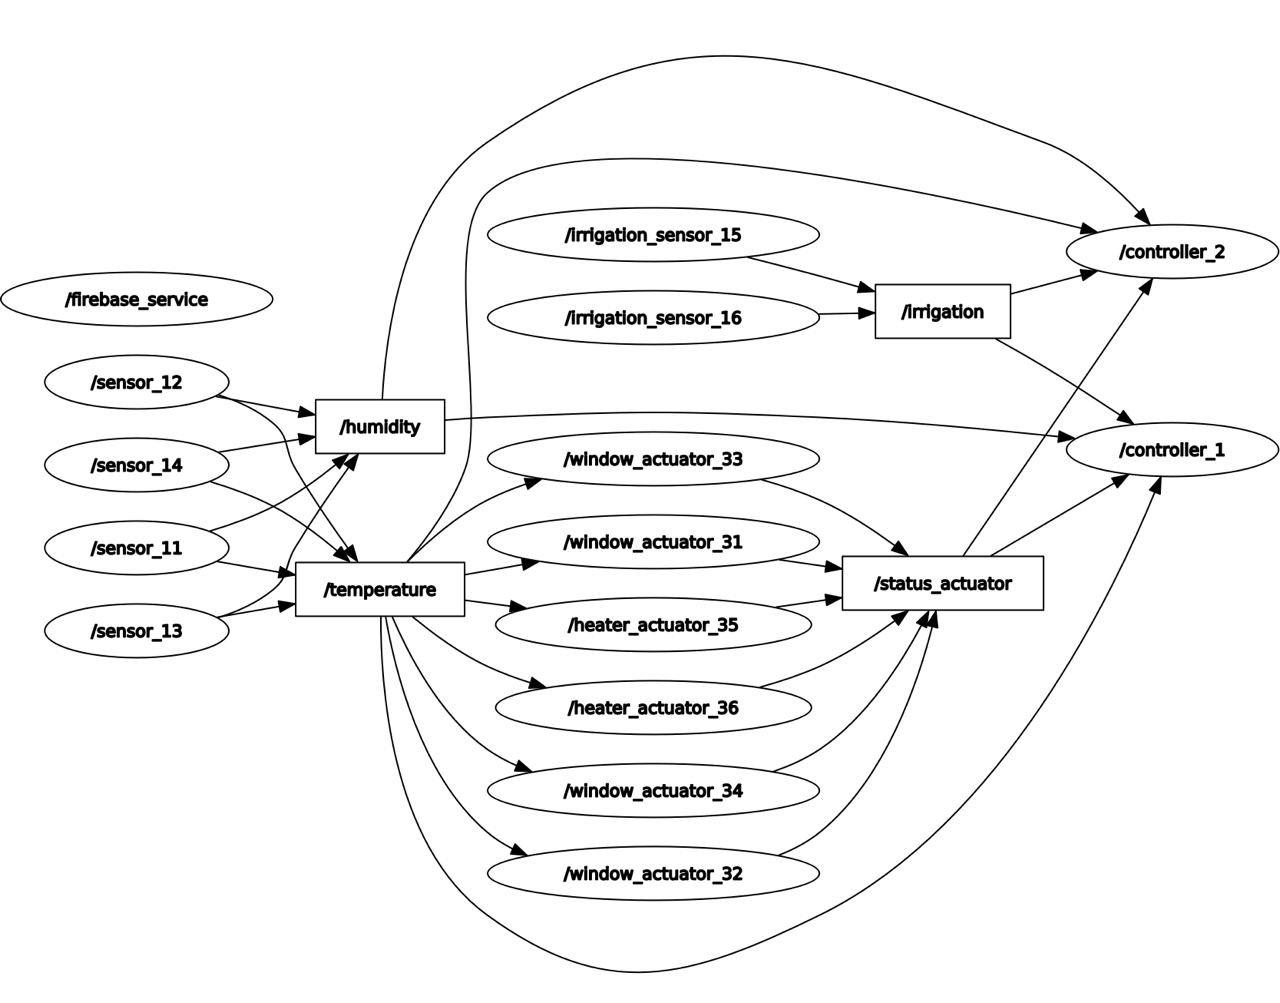
\includegraphics[width=\textwidth]{img/06-Rqt-graph.jpeg}
    \captionof{figure}{Simulación del escenario en la red}
    \label{fig:simulacion-escenario-nodos}
\end{center}

Al igual que en el anterior caso \ref{fig:rqt-graphs}, los óvalos son los nodos y los rectángulos los tópicos.

Este escenario ha sido desplegado utilizando los siguientes dispositivos:

\begin{itemize}
    \item \textbf{2 placas ESP32}, siendo los sensores 11 y 12, leyendo la información de los sensores DHT-11.
    \item \textbf{Raspberry Pi3B}, ejecutando uno de los controladores y almacenando los datos.
    \item \textbf{Portátil}, donde se ha desplegado los demás nodos con el \textit{launch file}.
\end{itemize}

\section{API REST para obtención de datos}

El desarrollo de esta API de comunicación estilo \ac{REST}, ha sido con el objetivo para poder tratar los datos y mostrarlos en la interfaz web explicada en la siguiente sección. Esta tecnología sirve para realizar de intermediario entre la base de datos y interfaz web.

Se van a destacar una serie de ventajas al usar API REST:

\begin{itemize}
    \item Hay una separación entre el cliente y el servidor, en este caso los usuarios que utilicen la interfaz y el servidor que contiene la base de datos.
    \item Hace más flexible el entorno de trabajo, ya que esta es independiente al tipo de lenguaje utilizado
    \item El manejo de errores respecto al acceso es gestionado por estas
\end{itemize}

Se puede destacar que en el caso de que se cambie de base de datos, ya que se han implementado dos, solo haya que modificar esta API y no sea necesario hacer ningún cambio en esa interfaz. Además, si se quiere utilizar los datos con fines relacionados con la inteligencia artificial, es más viable la conexión para poder analizar estos datos y aplicar algoritmos de entrenamiento o cálculos estadísticos.

Esta ha sido implementada en Python y con el framework FastAPI \cite{fastapi}. Esta tecnología ha sido utilizada para el desarrollo debido a que el despliegue es muy rápido, y en el caso de querer dockerizar este apartado y poder ejecutarlo en diferentes entornos es bastante simple.

Respecto al funcionamiento, este ejecuta Uvicorn \cite{uvicorn} que es un servidor ligero \ac{ASGI} para que este continuamente operativo este servicio.

\section{Interfaz Web}

Respecto a la interfaz a establecer, se ha seleccionado Angular \cite{angular} debido a la flexibilidad, robustez y la disponibilidad del uso de plantillas en comparación a otras alternativas como React o Vue. Además con planteamiento futuro, se podría implementar junto al framework de Ionic para creación de aplicaciones híbridas, pudiendo crear al finalizar una app para los sistemas operativos móviles como IOS y Android.

Angular utiliza \textit{Components}, que son encapsulaciones de código HTML, CCS y Javascript, dividiendo las diferentes estructuras comentadas en la figura \ref{fig:home} para un mejor diseño.

En Angular se ha utilizado Material \cite{material-angular} para el diseño de los diferentes elementos de la web. Material es un conjunto de componentes dotando de diseño y diferentes funcionalidades para hacer más cómodo y rápido esta parte con Angular. Gracias a que la documentación es muy completa y posee multitud de ejemplos, se puede adoptar en el proyecto para las diferentes secciones planteadas.

Para la conexión con la API, es necesario crear un \textit{service} en angular, que genere un \textit{Observable} para recibir la información de manera asíncrona. Este será utilizado en los componentes necesarios, pidiendo los diferentes tipos de datos.

Los componentes finalmente implementados han sido los siguientes:

\subsection{Home}

Este componente de la figura \ref{fig:home-final} muestra cada nodo de la red desplegada con la última información recopilada por este. Es la primera página que se va a visualizar a la plataforma, por lo que tiene que tener la parte esencial de estos datos.


\begin{center}
    \centering
    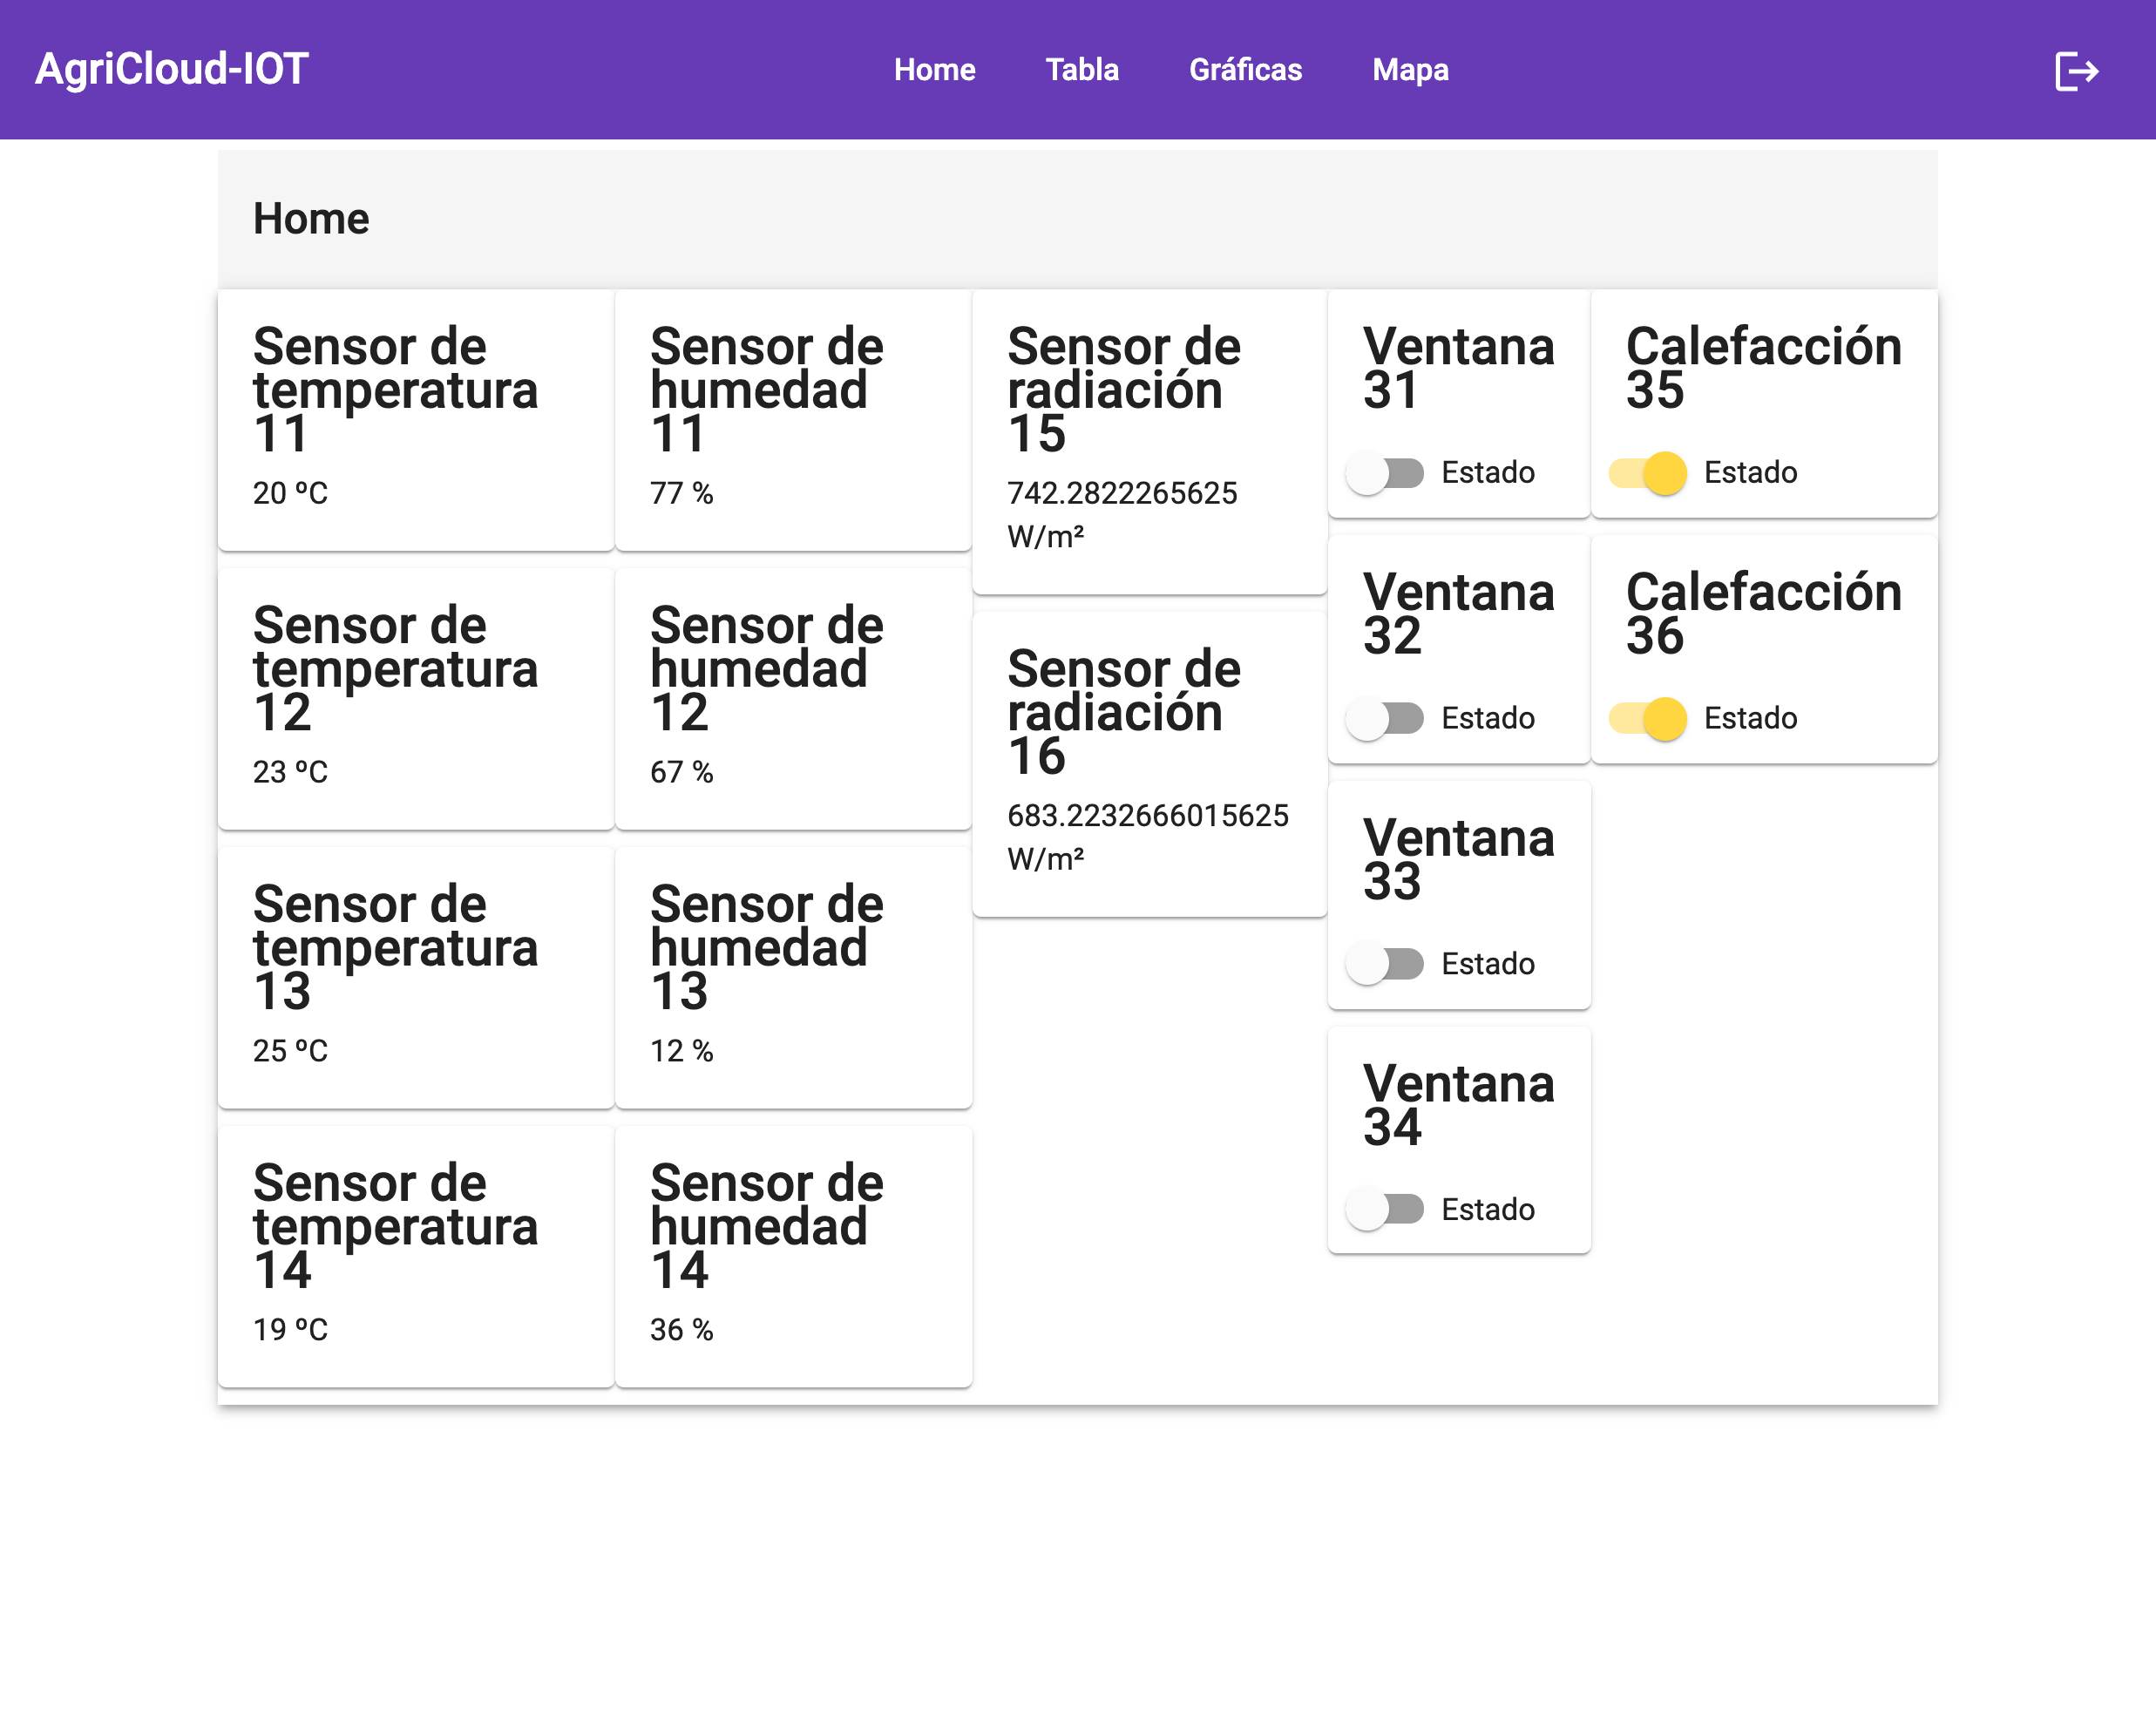
\includegraphics[width=0.8\textwidth]{img/06-Web-home.png}
    \captionof{figure}{Página principal}
    \label{fig:home-final}
\end{center}

\subsection{Tabla de datos}

Respecto a la tabla de datos, esta ha implementado paginación para una visualización más cómoda, posibilidad de ordenamiento de los datos según cada cabecera o filtrado de estos datos.

Por lo tanto, en el caso de se que quiera buscar por una hora, se escribiría en el filtro la hora, o si se quiere ordenar de mayor a menor tomando como referencia el tiempo, solo sería necesario hacer click en esa columna.

\newpage

\begin{center}
    \centering
    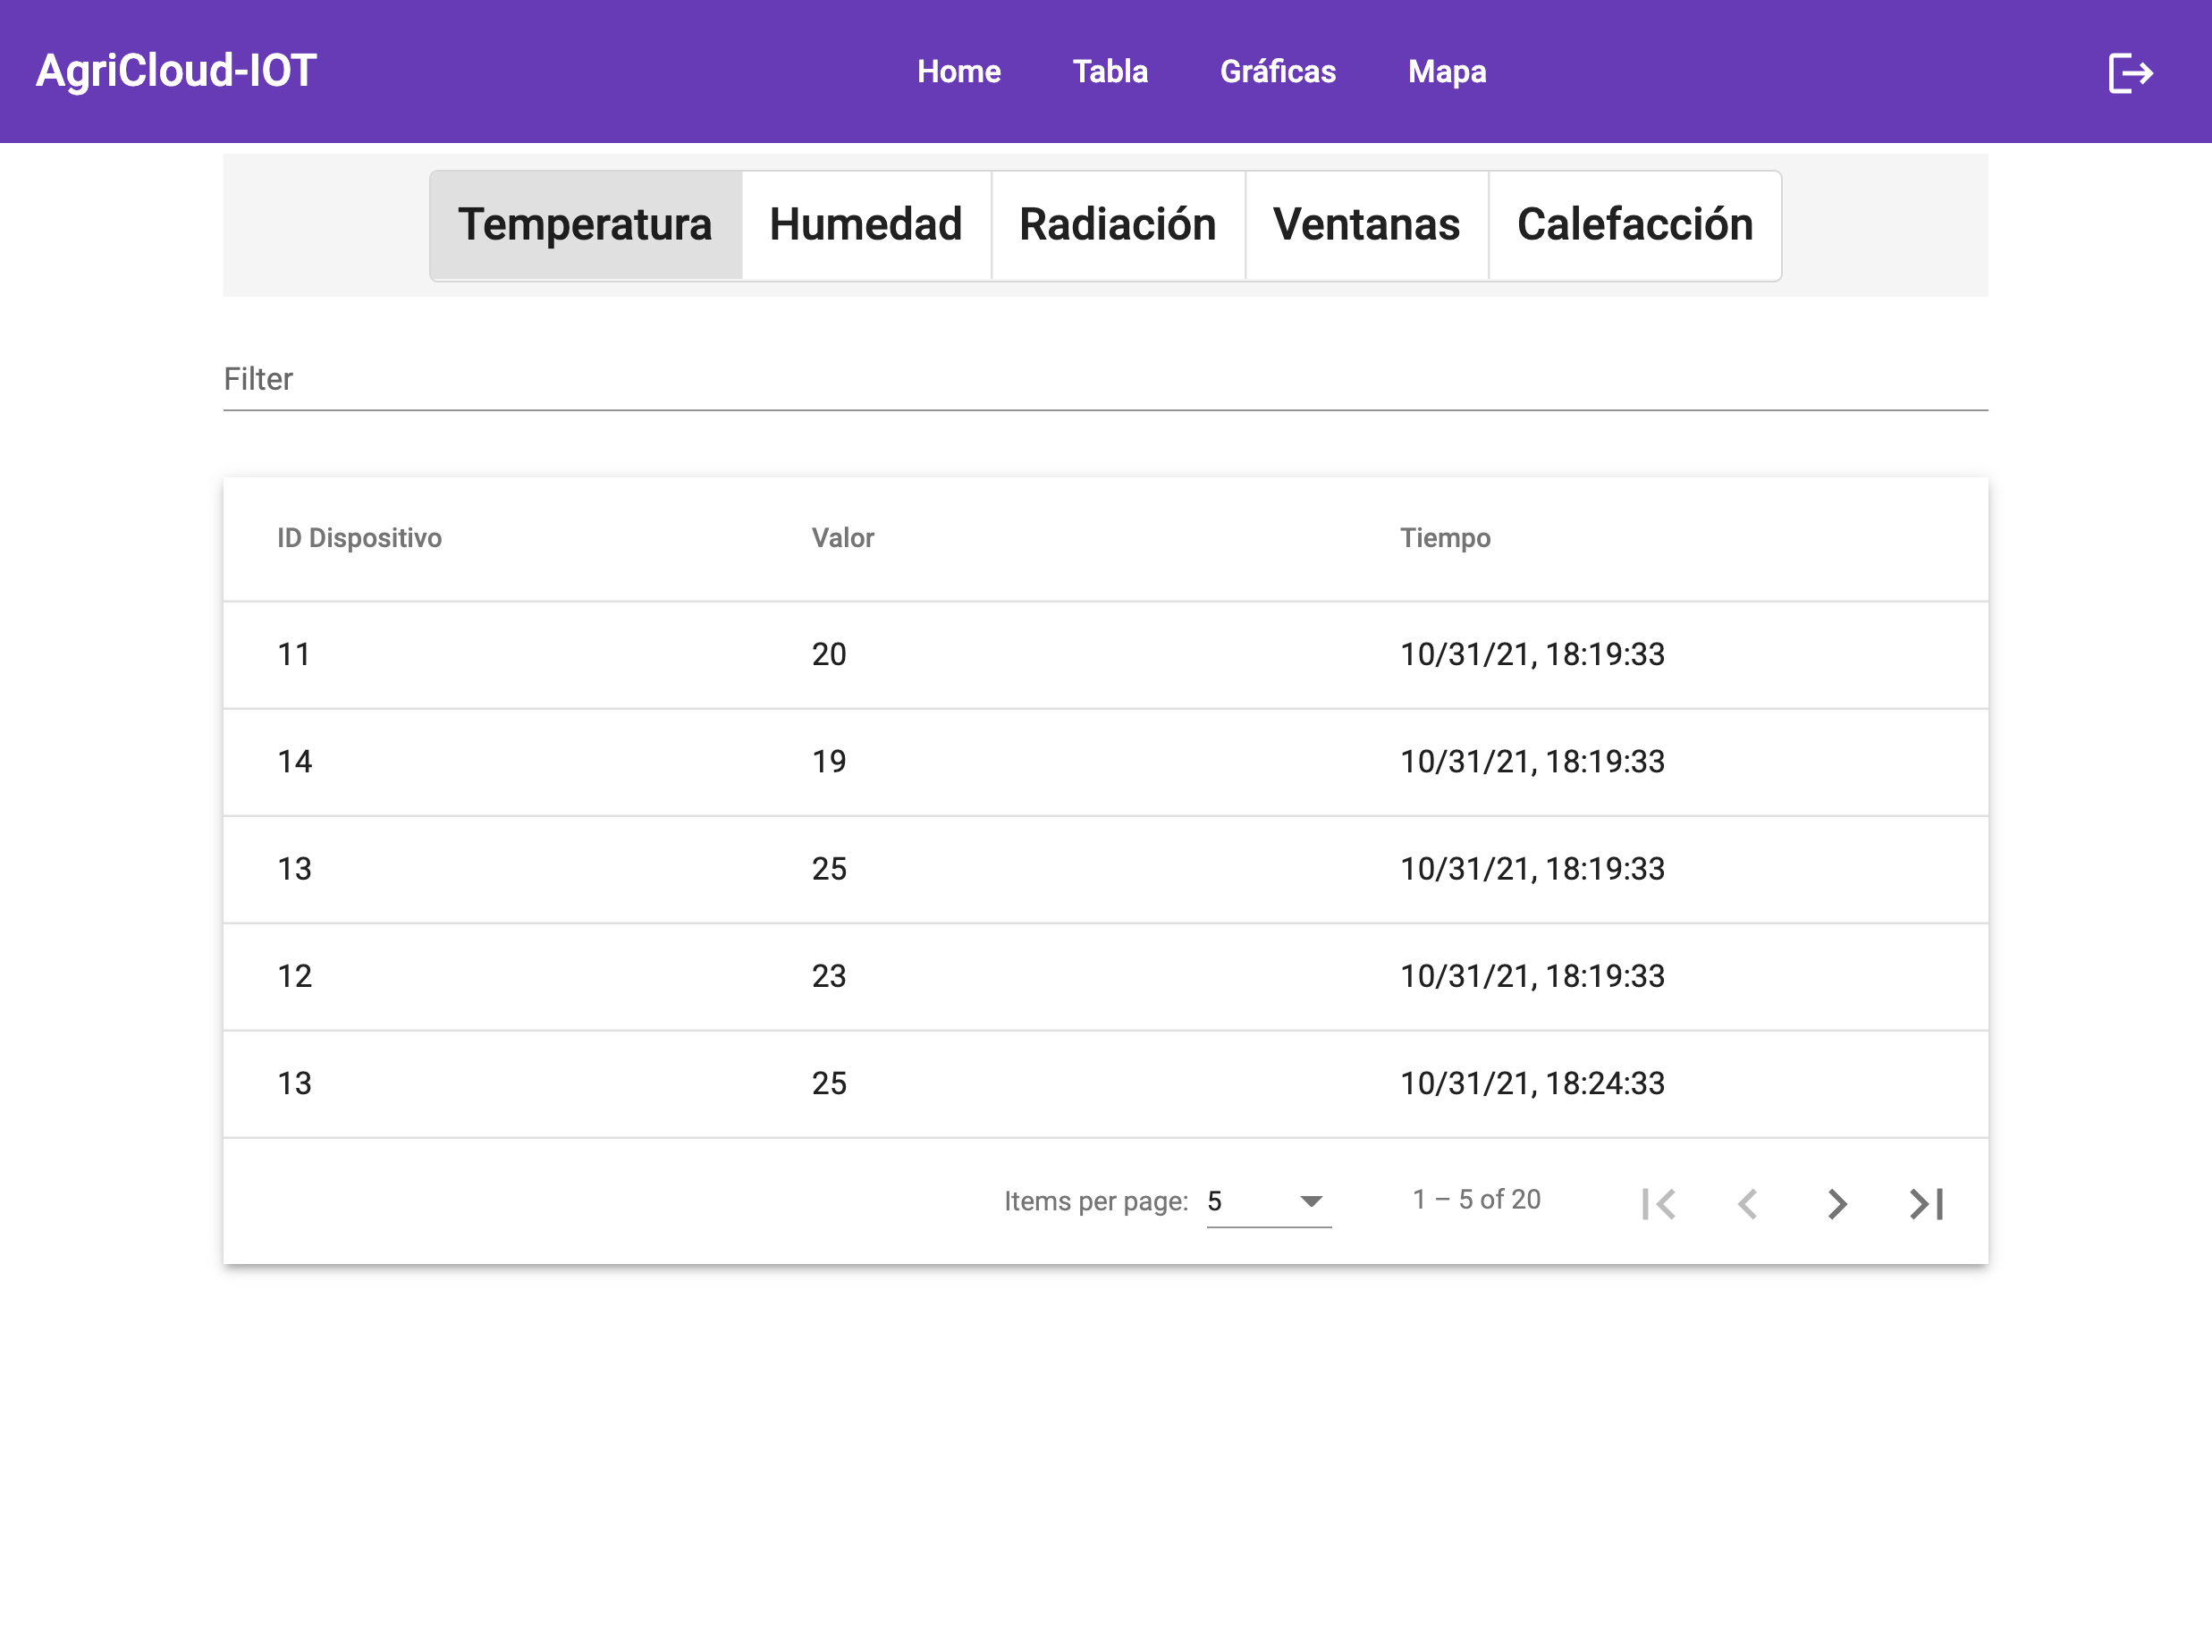
\includegraphics[width=0.8\textwidth]{img/06-Web-tablas.png}
    \captionof{figure}{Tablas de datos}
    \label{fig:tablas-de-datos-final}
\end{center}

\subsection{Gráficos}

Esta sección hace uso de Google Charts \cite{charts-google}, en concreto un paquete disponible para Angular publicado en Github.

Se han escogido las gráficas tipo lineal ya que permiten de un vistazo ver los cambios en los datos producidos en los diferentes sensores.

\begin{center}
    \centering
    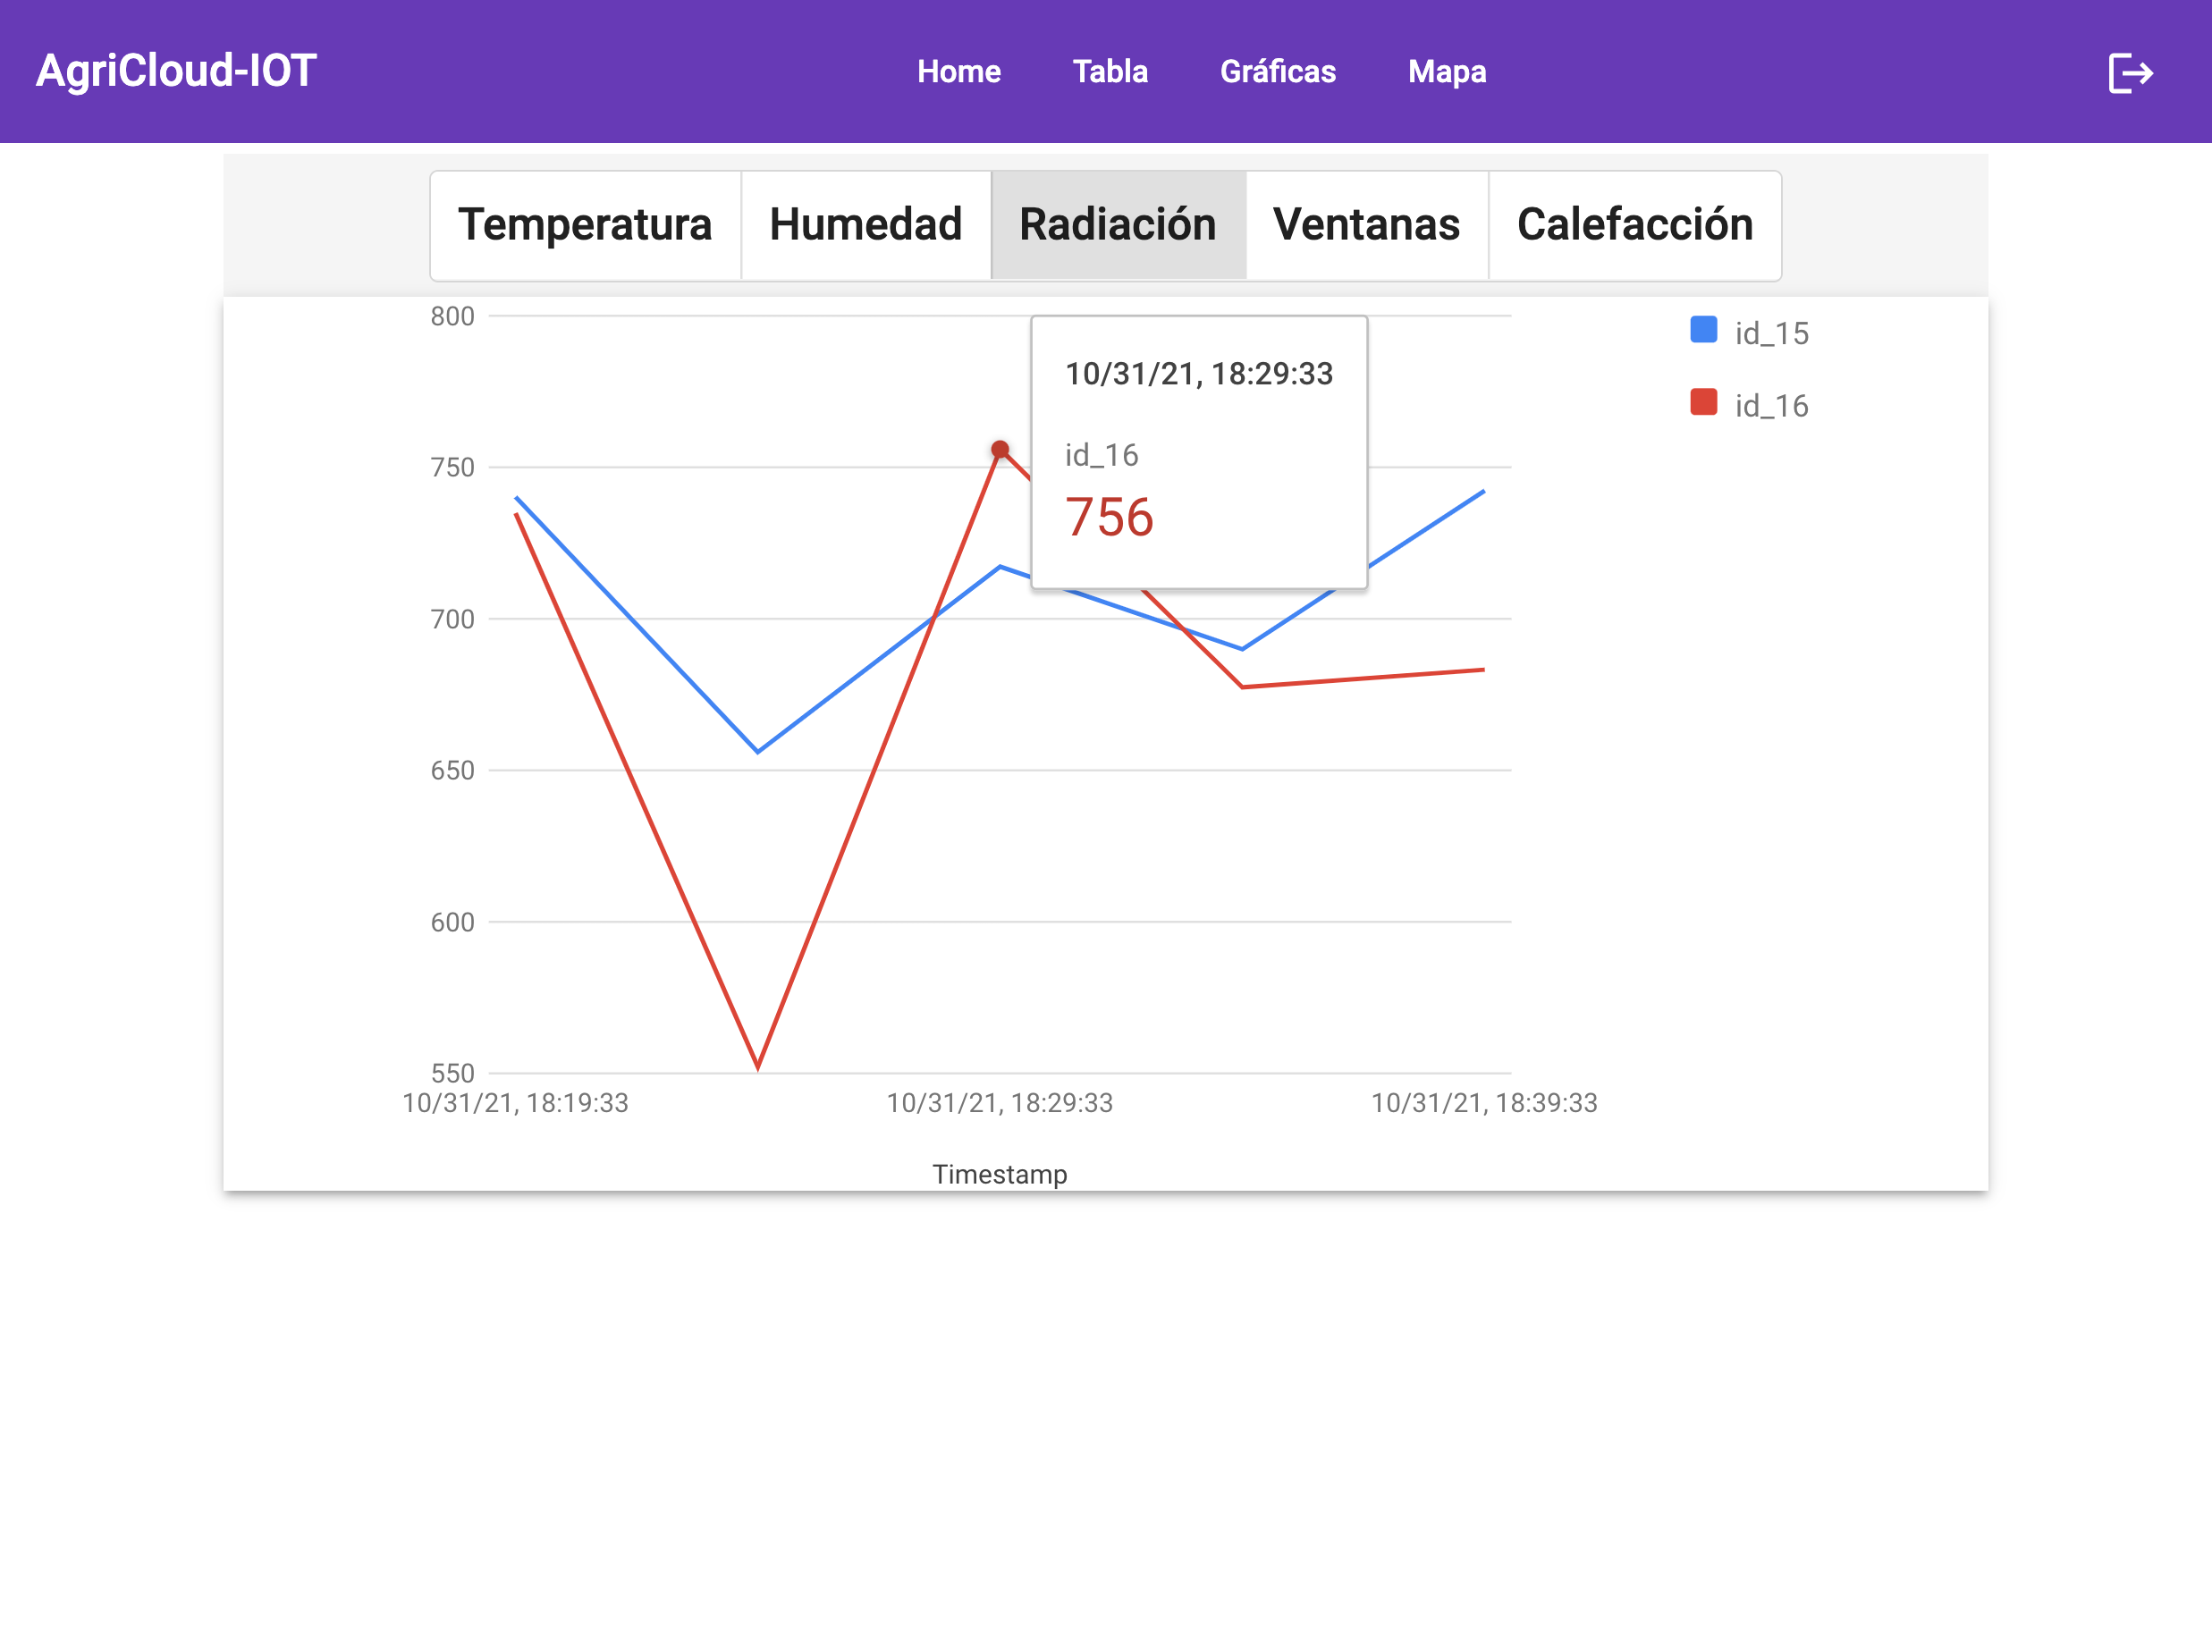
\includegraphics[width=0.8\textwidth]{img/06-Web-charts.png}
    \captionof{figure}{Gráficas de radiación}
    \label{fig:graphs-final}
\end{center}


\subsection{Mapa}

En la imagen \ref{fig:mapa-final} se muestra el mapa final, similar al mostrado en la figura del capítulo de análisis \ref{fig:mapa}, para que el usuario que acceda pueda visualizar la posición de cada nodo, además de poder obtener los datos de este al seleccionarlo, mostrados en el recuadro superior.

\begin{center}
    \centering
    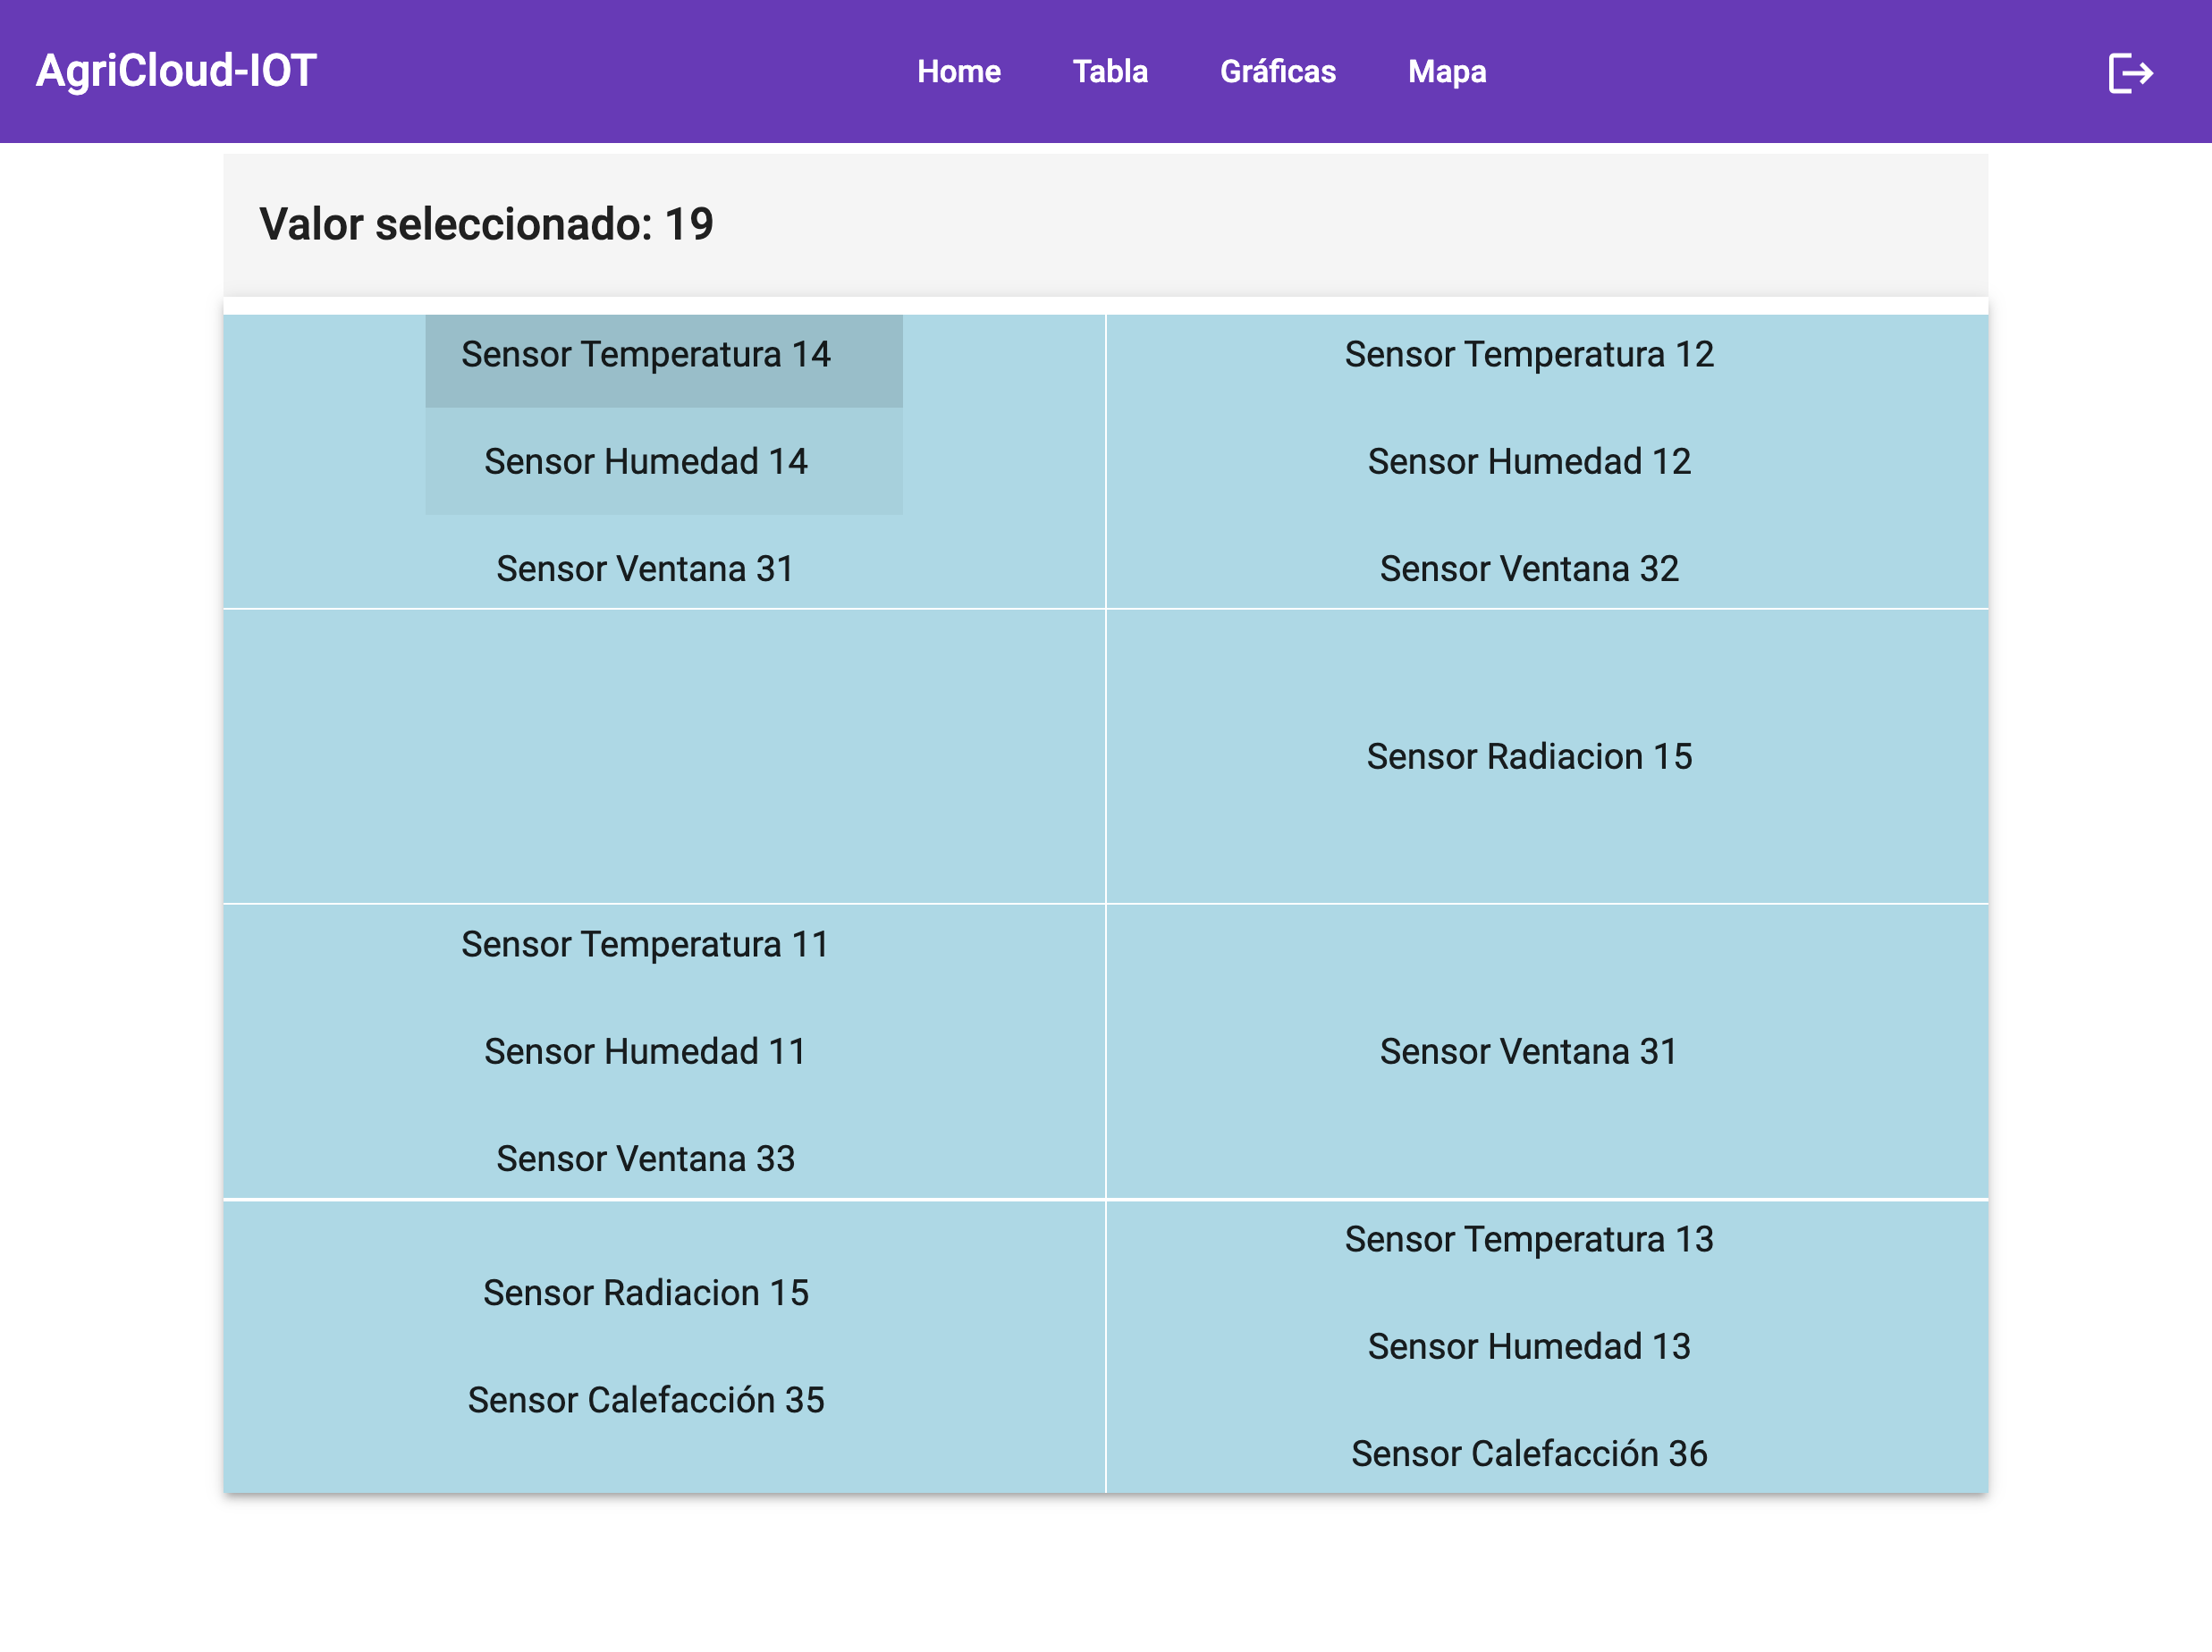
\includegraphics[width=0.8\textwidth]{img/06-Web-map.png}
    \captionof{figure}{Mapa interactivo con los diferentes sensores}
    \label{fig:mapa-final}
\end{center}

\newpage

\subsection{Login}

Se ha querido dejar hecho una página de inicio de sesión, ya que a lo largo de la implementación de la interfaz web, se ha planteado el acceso de diferentes usuarios a esta plataforma.

Por ello se muestra en la siguiente captura \ref{fig:login-final} la introducción de las credenciales de usuario.

\begin{center}
    \centering
    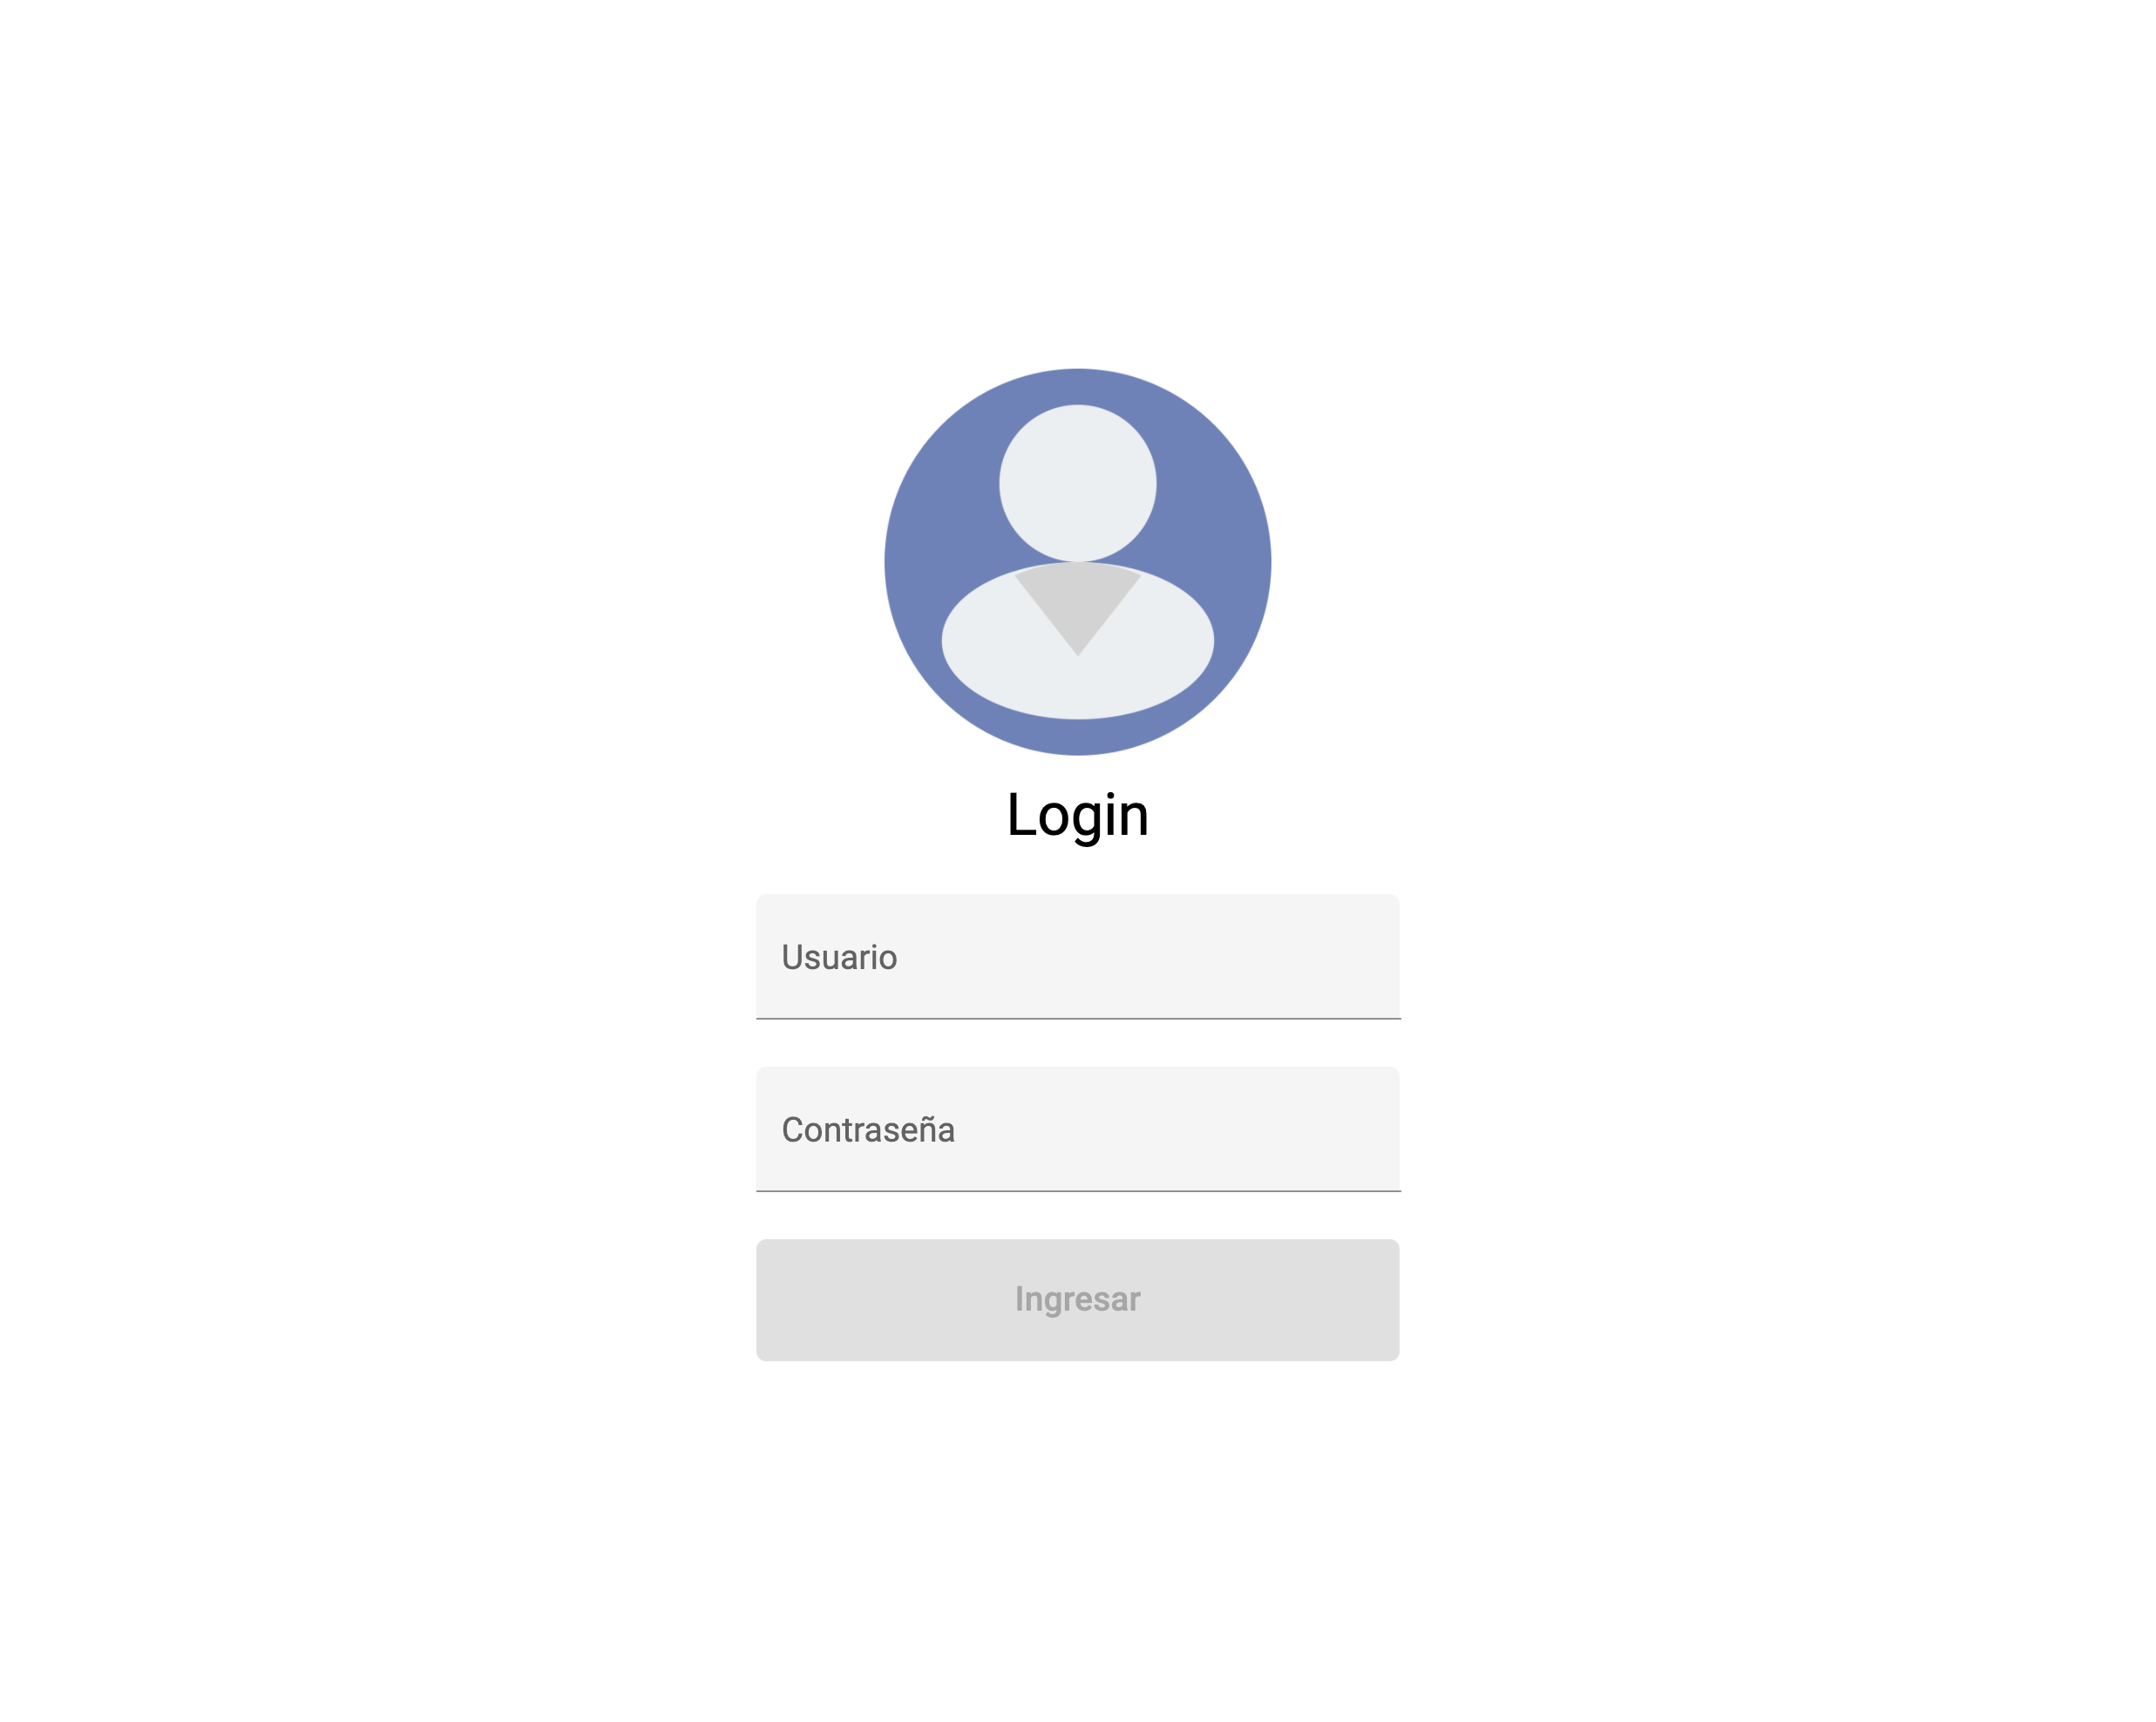
\includegraphics[width=0.8\textwidth]{img/06-Web-login.png}
    \captionof{figure}{Login implementado}
    \label{fig:login-final}
\end{center}

Esta podría ser la página principal de nuestra interfaz, y tras introducir nuestras credenciales ya se muestre el Home correspondiente a ese usuario.